\begin{frame}{¿Quién soy?}


\includegraphics{../figures/talk/twitter.png}

\end{frame}

\begin{frame}{Les invito ser voluntarias de Software Carpentry como yo}

Desarrollamos lecciones en colaboración y enseñamos talleres en todo el
mundo

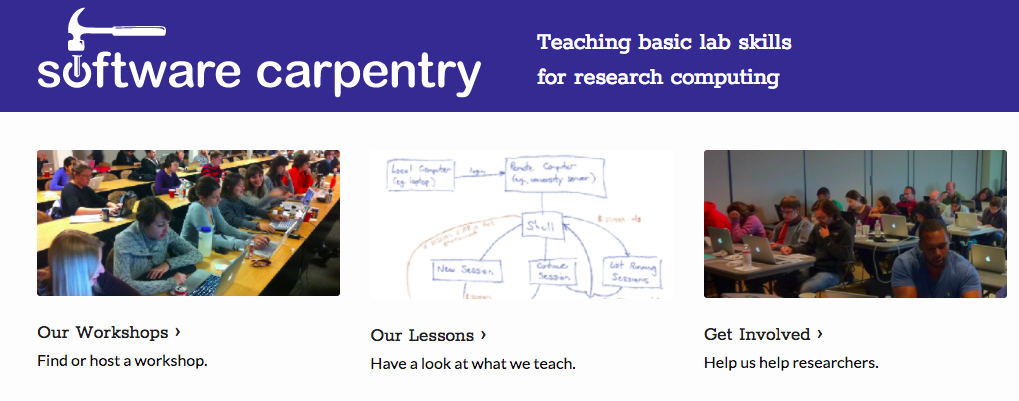
\includegraphics{../figures/talk/swc.png}

Imagen de \url{https://software-carpentry.org/}

\end{frame}

\begin{frame}{Cosas que aprendií que quiero compartir}

\begin{itemize}[<+->]
\tightlist
\item
  Todos somos terribles al principio
\item
  La mejor manera de aprender es a ensenñar
\item
  Todos aprenden más cuando la ciencia y la educación están abiertas
\end{itemize}

\end{frame}

\begin{frame}{Consejo 3: Usa R notebooks para la reproducibilidad}

\end{frame}

\begin{frame}{Consejo 4: Usa el control de versiones para la
colaboración}

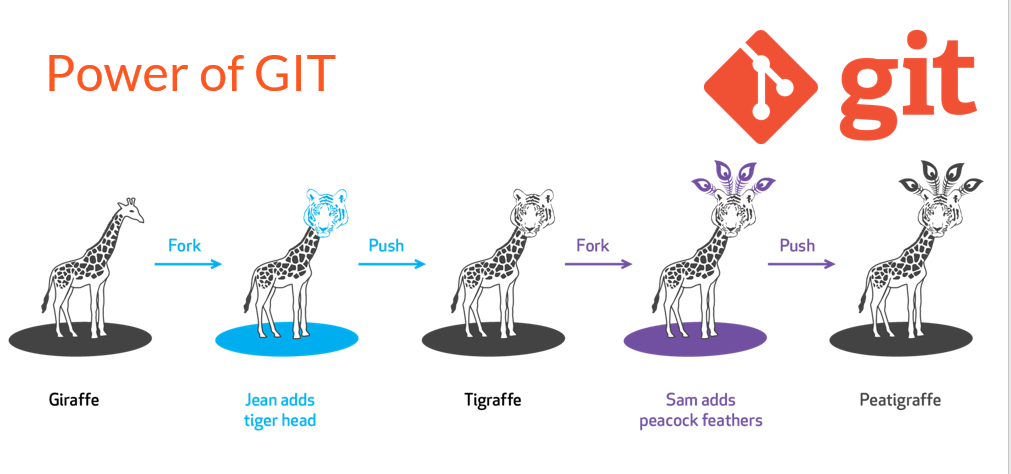
\includegraphics{../figures/talk/git-graphic-01.png}

\end{frame}

\begin{frame}{Consejo 5: Documente su flujo de trabajo}

\includegraphics{https://www.blogdelfotografo.com/wp-content/uploads/2016/05/mark-516279_1920.jpg}

\url{https://www.blogdelfotografo.com/workflow-flujo-trabajo-foto/}

\end{frame}

\begin{frame}{Por ejemplo, puede enumerar los comandos por orden de
operación}

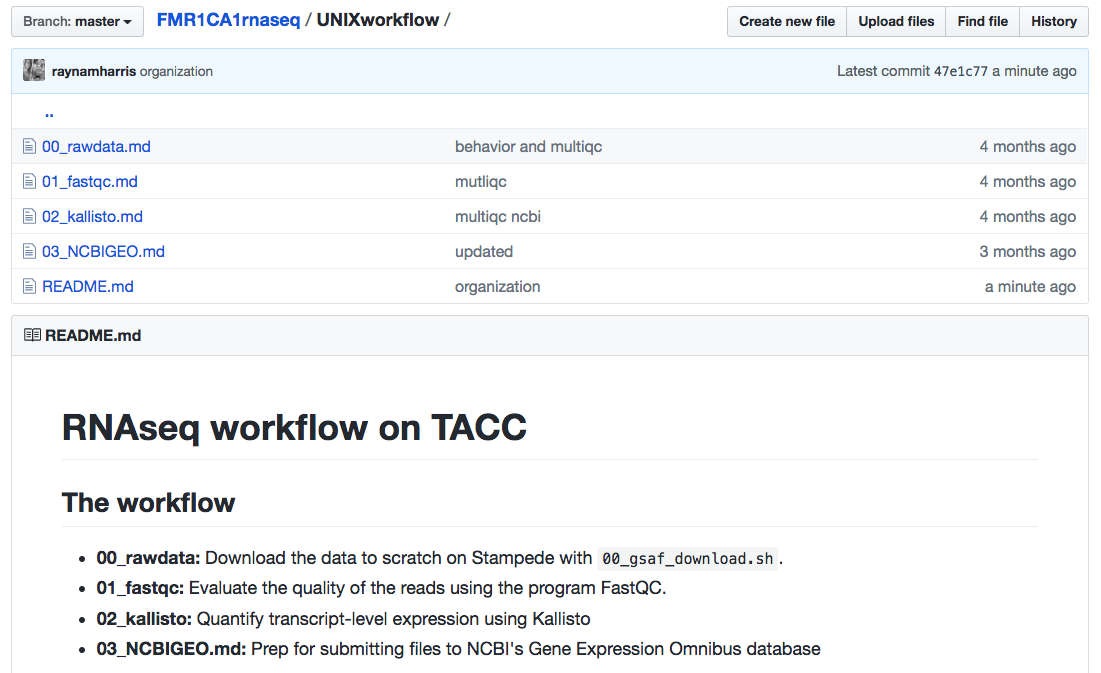
\includegraphics{../figures/talk/unixworkflow.png}

Imagen de \url{https://github.com/raynamharris/FMR1CA1rnaseq-ES}

\end{frame}

\begin{frame}{Pruebe múltiples estrategias de organización y haga lo que
funcione mejor para vos}

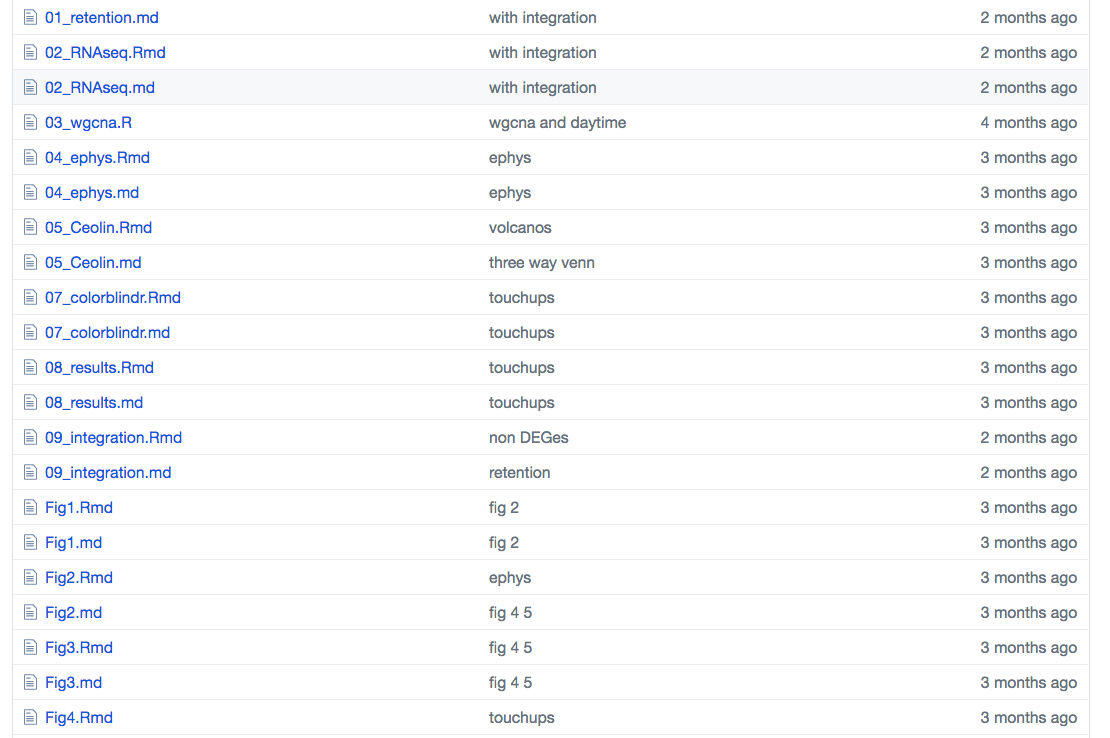
\includegraphics{../figures/talk/Rworkflow.png}

Imagen de \url{https://github.com/raynamharris/FMR1CA1rnaseq-ES}

\end{frame}

\begin{frame}{Esperanza: que uses colores personalizados}

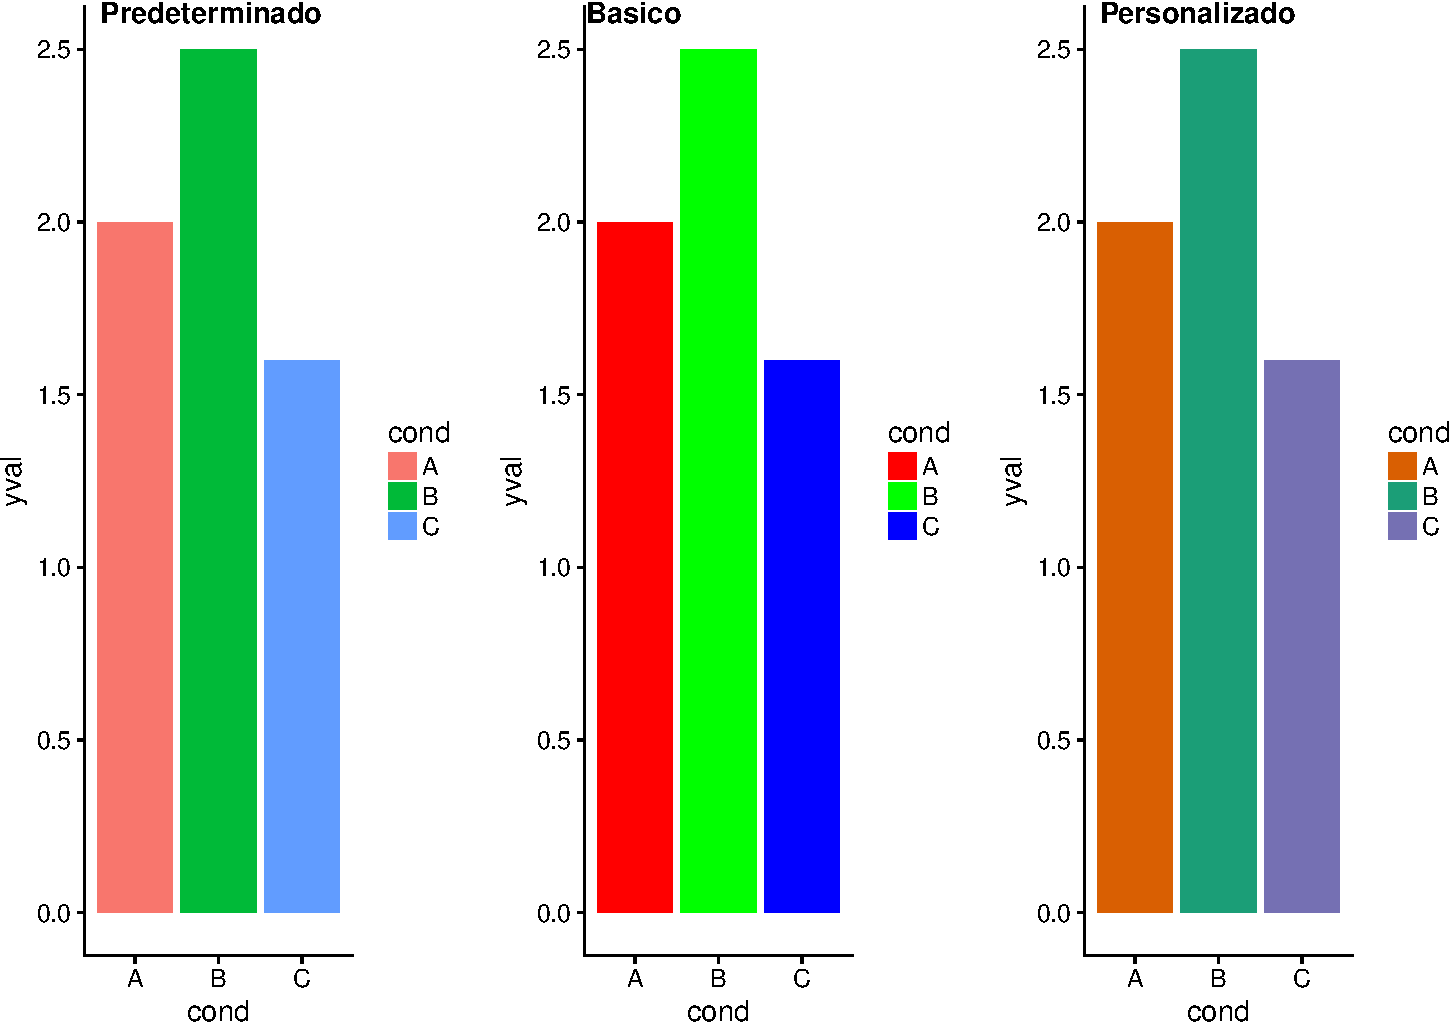
\includegraphics[width=250px]{../figures/talk/unnamed-chunk-1-1}

I: predeterminado

II: values=c(``red'', ``green'', ``blue'')

III: values=c(``\#CC6666'', ``\#66CC99'', ``\#9999CC'')

\end{frame}

\begin{frame}{Consejo 6: Desarrolla tu propia paleta de colores}

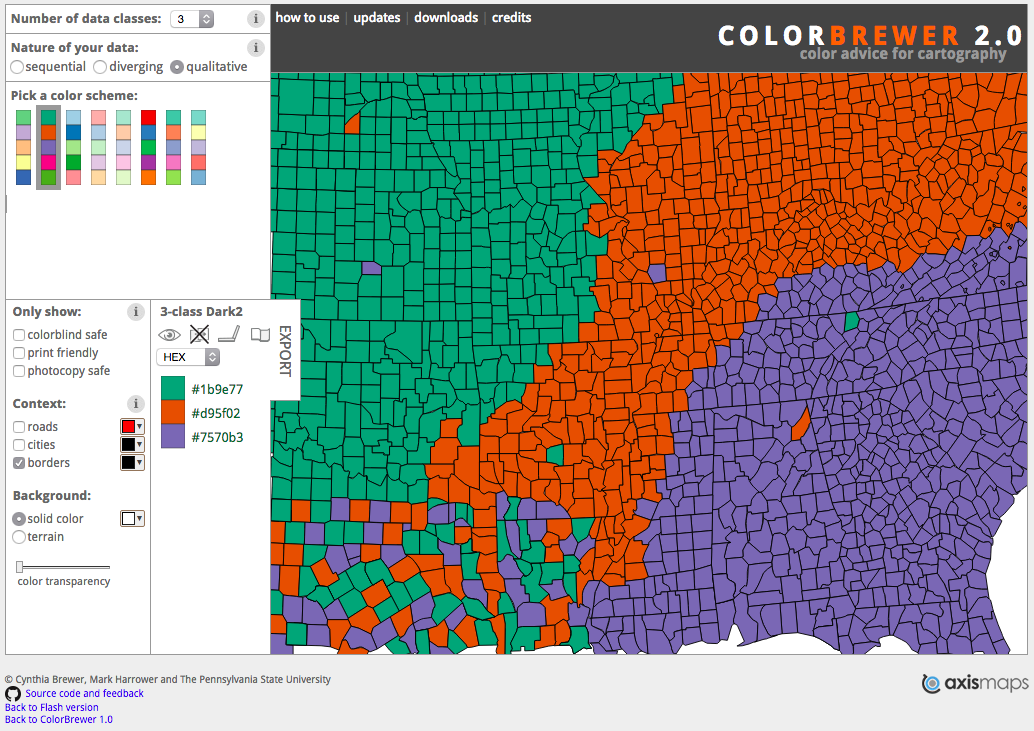
\includegraphics{../figures/talk/colorbrewer.png}

Imagen de \url{http://colorbrewer2.org/}

\end{frame}

\begin{frame}{Consejo 7: Leyendas graficas son joyas}

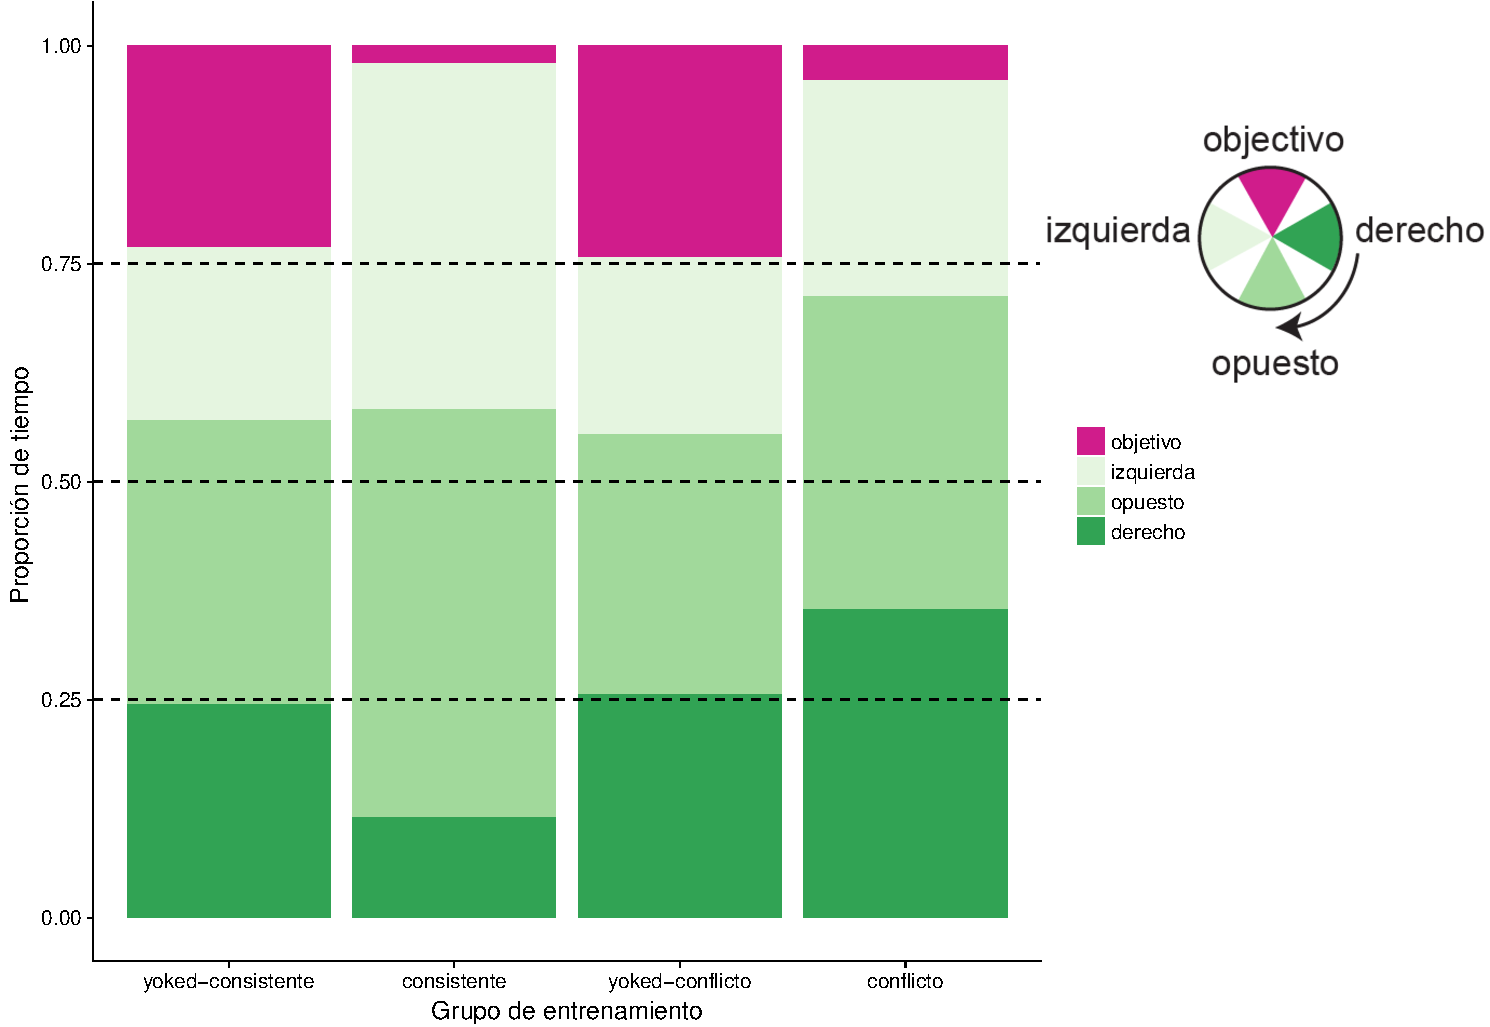
\includegraphics{../figures/talk/timespent-1.pdf}

\url{https://cran.r-project.org/web/packages/cowplot/index.html}

\end{frame}

\begin{frame}{Consejo 8: Comparte tu trabajo}

\end{frame}

\begin{frame}{Consejo 9: Promover tu trabajo}

\end{frame}

\begin{frame}{Consejo 1: Nunca enseñes sola}

\end{frame}

\begin{frame}{Consejo 2: Desarrolla lecciones en colaboración}

Citation: Devenyi GA, Emonet R, Harris RM, Hertweck KL, Irving D,
Milligan I, et al. (2018) Ten simple rules for collaborative lesson
development. PLoS Comput Biol 14(3): e1005963.
\url{https://doi.org/10.1371/journal.pcbi.1005963}

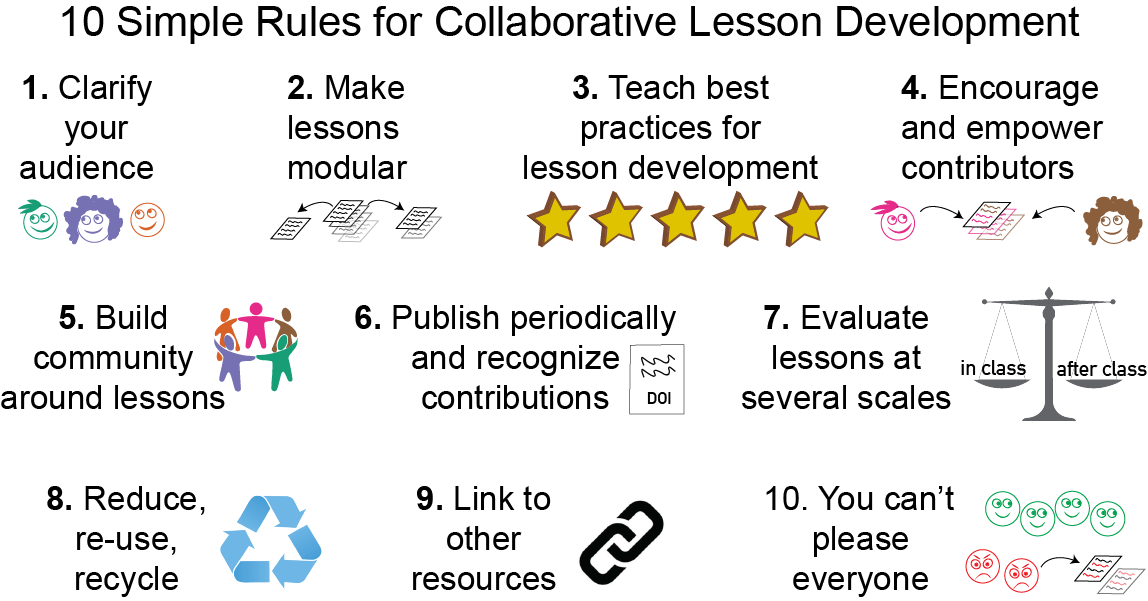
\includegraphics{../figures/talk/plos.png}

\end{frame}
